% Created 2023-06-04 Sun 16:38
% Intended LaTeX compiler: pdflatex
\documentclass[9pt, b5paper]{article}
\usepackage{xeCJK}
\usepackage[T1]{fontenc}
\usepackage{bera}
\usepackage[scaled]{beraserif}
\usepackage[scaled]{berasans}
\usepackage[scaled]{beramono}
\usepackage[cache=false]{minted}
\usepackage{xltxtra}
\usepackage{graphicx}
\usepackage{xcolor}
\usepackage{multirow}
\usepackage{multicol}
\usepackage{float}
\usepackage{textcomp}
\usepackage{algorithm}
\usepackage{algorithmic}
\usepackage{latexsym}
\usepackage{natbib}
\usepackage{geometry}
\geometry{left=1.2cm,right=1.2cm,top=1.5cm,bottom=1.2cm}
\usepackage[xetex,colorlinks=true,CJKbookmarks=true,linkcolor=blue,urlcolor=blue,menucolor=blue]{hyperref}
\newminted{common-lisp}{fontsize=\footnotesize} 
\author{deepwaterooo}
\date{\today}
\title{ET 框架学习笔记(二)--网络交互相关}
\hypersetup{
 pdfauthor={deepwaterooo},
 pdftitle={ET 框架学习笔记(二)--网络交互相关},
 pdfkeywords={},
 pdfsubject={},
 pdfcreator={Emacs 28.2 (Org mode 9.5.5)}, 
 pdflang={English}}
\begin{document}

\maketitle
\tableofcontents


\section{写在最后:反而是自己每天查看一再更新的}
\label{sec:orgd540648}
\begin{itemize}
\item 【问题】:上次那个ET-EUI 框架的时候,曾经出现过 opcode 不对应,也就是说,我现在生成的进程间消息,有可能还是会存在服务器码与客户端码不对应,这个完备的框架,这次应该不至于吧?
\item 【UIType】部分类:这个类出现在了三四个不同的程序域,现在重构了,好像添加得不对。要再修改
\end{itemize}

\section{现在的修改内容:【任何时候,活宝妹就是一定要嫁给亲爱的表哥!!!爱表哥,爱生活!!!】}
\label{sec:org3635ac2}
\begin{itemize}
\item \textbf{【ET7 框架】} 没有处理的逻辑是: \textbf{【ET7 框架里数据库的接入】}
\item \textbf{【Windows 下 proto2cs 消息转化】} : ProtoBuf 这个库里还存在几个问题, enum-repeated 等关键字,因为程序域的问题等,没能连能
\item \textbf{【UILobbyComponent 可以测试】} :这个大厅组件,Unity 里预设简单,可以试运行一下,看是否完全消除这个UI 组件的报错,这个屏的控件能否显示出来?还是错出得早,这个屏就出不来已经报错了?
\begin{itemize}
\item 【客户端】的逻辑是处理好了,编译全过后可以测试
\item 【服务端】:处理用户请求匹配房间的逻辑,仍在处理: \textbf{C2G\_StartMatch\_ReqHandler}.
\end{itemize}
\item \textbf{【TractorRoomComponent】} :因为是多组件嵌套,可以合并多组件为同一个组件;另早上看得一知半解的一个【ChildOf】标签,可以帮助组件套用吗?再找找理解消化一下
\item 【房间组件】:几个现存的 working-on 的问题:
\begin{itemize}
\item 多组件嵌套:手工合并为一个组件。彻底理解确认后,会合并
\item 【服务端】:处理用户请求匹配房间的逻辑. 这里的编译错误终于改完。到时就看运行时错误了。
\begin{itemize}
\item 【数据库模块的整合】:网关服在转发请求匹配时,验证会话框有效后,验证用户身份时,需要去【用户数据库】拿用户数据。ET7 留了个DBManagerComponent, 还没能整合出这个模块
\end{itemize}
-【参考来源 \textbf{C2R\_LoginHandler} 】:Realm 处理客户端的登录请求的服务端逻辑。这里看见,它随机分配一个网关服。也就是,我(原本本质上也是随机分配)一个匹配服给用。可以依照这里的例子来改写。
\end{itemize}
\item \textbf{【服务端的编译错误】} 基本上扫了一遍。【客户端】因为这些前期的工作,以及拖拉机项目重构设计还没有想透彻,暂停一下。
\item 【接下来的内容】: \textbf{【重构拖拉机项目】} 。把ET7 框架里【参考项目】的设计看懂,并借助这个例子,把拖拉机项目设计好。
\item 有时间,会试着尽早解决上面 ProtoBuf 里的几个小问题。但现在需要重构的设计思路,客户端的界面等才能够往下进行。 
\begin{itemize}
\item 【匹配服地址】网关服的处理逻辑里,验证完用户合格后,为代为转发消息到匹配服,但需要拿匹配服的地址。ET7 重构里,还没能改出这部分。服务器系统配置初始化时,可以链表管理各小构匹配服,再去拿相关匹配服的地址。ET7 框架里的路由器系统,自己还没有弄懂。
\item 这个地方有点儿脑塞,完全搜不到新框架里可以参考的例子,暂时写不到了。那可以去读一读更大的框架,去找别人用ET7 的别人的例子里是怎么写的,再去参考一下别人的。【爱表哥,爱生活!!!任何时候,活宝妹就是一定要嫁给亲爱的表哥!!!】今天下午先去看 Tractor 游戏源码,设计重构思路
\end{itemize}
\item 这些要找的也找不到。下午家里试着把Component 组件再添加回去试试看 \textbf{【不能再添加Component 组件。ET7 框架重构了,小单元也走热更新,在热更新层有天文小行星的生成系。可以参照 ET.pdf 里的服务端 PlayerSystem 来作例子】} ?上午把项目设计的思路,源项目的破源码再读一读理一理,是希望游戏逻辑与游戏界面能够快速开发、项目进展往后移的。
\begin{itemize}
\item User.cs 客户端的话,不知道要不要修改。晚点儿的时候留意一下。
\item Gamer.cs 客户端保留了 Dispose
\end{itemize}
\item 还有 79 个小错误: protobuf 里还有小问题需要修改。先改了,一次把 Protobuf 里的小错误全部改完了。电脑没好好工作,前后文件不一致。。。。【活宝妹就是一定要嫁给亲爱的表哥!!!】爱表哥,爱生活!!!
\begin{itemize}
\item \textbf{【IScene】} :不知道哪里崩出来的神龙见首不见尾的,两处,还不知道怎么修改这个编译错误。。。不知道源码是什么原因,弄得乱七八糟,参照原版本的改正一下就可以了,因为现项目里根本就不存在这个的接口类。
\item 有些文件加了两遍:当我能够从VSC 里删除的时候,却无法从VS 里删除掉索引。找到VS 里可以看见文件的地主,感觉台式机真是慢,让我看见,已经是晚了 800 年了。。。【爱表哥,爱生活!!!任何时候,活宝妹就是一定要嫁给亲爱的表哥!!!】
\item 把还没有用到,但是报错了的几个类删掉:比如记一下: SessionInfoComponent,
\item PlayerComponent 狠奇怪:删除了说找不到类,不删除说重复了,感觉台式机应用有延迟?反应狠慢。。。。。
\item 还剩最后 26 个最挑战活宝妹的编译错误,今天傍晚会家里改会儿,集中问题明天上午希望能够看懂。【爱表哥,爱生活!!!任何时候,活宝妹就是一定要嫁给亲爱的表哥!!】
\end{itemize}
\end{itemize}

\begin{center}
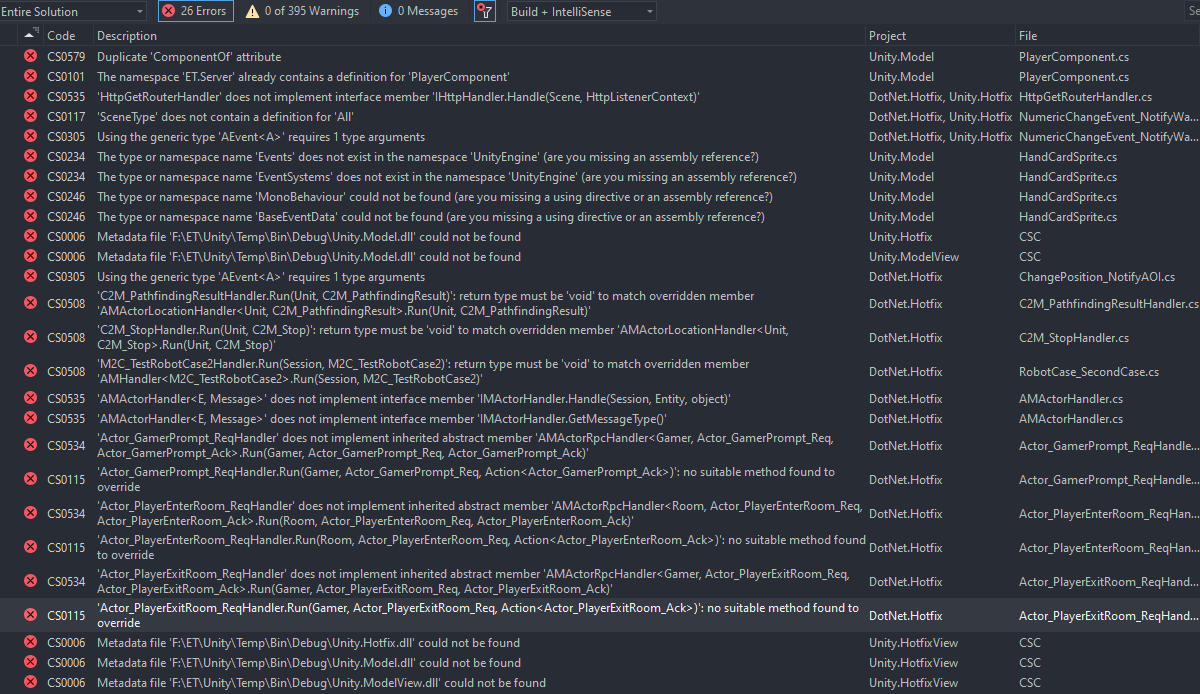
\includegraphics[width=.9\linewidth]{./pic/et4_20230604_162732.png}
\end{center}
\begin{itemize}
\item \textbf{ETTask-vs-ETVoid}: 框架里有狠多需要改的地方。今天上午的脑袋好使,把这块儿再仔细好好看下。今天上午把以前不懂的模块都稍微看下,再理解一下
\begin{itemize}
\item 查网页感觉也查不出什么来。还是用源码帮助理解概念。今天晚上整理一下这一块儿,把这个问题弄明白了。【爱表哥,爱生活!!!活宝妹就是一定要嫁给亲爱的表哥!!!】
\item 不能把所有基类的 async ETTask 返回参数直接改成 void, 因为框架的顶层应用,服务端或是客户端,当不异步等待结果,如资源包没能下载完成,就接着往下执行,会报空异常。
\end{itemize}
\item 现在的问题是:Protobuf 里 repeated 关键字,好像还是没有处理好,找不到成员变量  Cards. 是因为 Proto2CS 的时候,确实把 repeated 关键字给处理丢了。因为我的 .proto 文件里有错误。(这就是上面先前觉得奇怪的原因。因为改这个的过程中把那些错改正了,就可以生成成功并找到相关的消息了)。
\item \textbf{【HandCardSprite 这个最近要弄明白】} 不知道这个类是为什么,整了一堆的错误,它是ETModel 里的。感觉是常规域,没弄明白为什么常规域还有ILRuntime 的适配呢?
\begin{itemize}
\item 要把 ILRuntime 热更新第三库,也再弄得明白一点儿【今天上午把这里再看,最好是能够结合源码看看】为什么这个类还要适配ILRuntime ?
\item 这里这个类,整个框架里只找到这一个用的地方,所以它一定是添加在某个预设或是场景中的某个控件下的。只是参考项目的unity 客户端,我运行不到打牌的这个界面,就先因为抛出异常而淡能运行。所以还没能找到哪个预设或是场景中的哪个控件添加了这个类,但是当然一定是跟玩家手牌相关的。 \textbf{【HandCardSprite 是在 handcard 预设里添加了这个脚本】}
\item 这个类今天运行狠奇怪,VS022 里找不到了。。。就是说,VSC 里它是在Model 客户端的源码里,但是从VS 里打开,找不到这个类文件所在的文件夹和文件,没有索引好,再添加一下?
\item 那么,为什么前两天被这个 block 住,而那天,好像是有删除掉这个文件,但文件夹应该是还在的才对呀?我可能还会试着再把它添加回去。
\item 但是,会在把当前几个编译错误改完,试着测试一下客户端现在有的界面之后,再试着添加回去,整理和 develop TractorRoomComponent 界面的内容。【爱表哥,爱生活!!!活宝妹任何时候就是一定要嫁给亲爱的表哥!!】
\item 今天下午家里再运行一次,当客户端抛异常,应该是某个热更新的资源包没有找到什么的?所以可以试着自己去解决这个客户端实时运行时抛出的异常。
\item \textbf{【参考项目斗地主客户端异常】} :再运行一次,试着分析,是否可以 unity 里实时运行,如果不可以,为什么不可以?
\begin{itemize}
\item 应该是LandlordsRom 这个预设与UI 类型没能连接起来,也就是找不到这个预设。
\item 那为什么打好包的可以呢?因为打好包的预设包名 LandlordsRoom.unity3d 与游戏逻辑契合,可以找得到
\item 可是仍然感觉奇怪:LandlordsLogin 与LandlordsLobby, 非常类似都可以找到,为什么就LandlordsRoom 找不到?可能LandlordsRoom 预设还是有某点儿物对特殊的地方。
\item 上面这个暂时跳过。现在仍然主要去看HandCardSprite 为什么参考项目里可以,而ET7 里就不可以。
\end{itemize}
\item 就是上面那个异常,今天下午得去弄明白,为什么只在 unity 实时运行时会抛异常,而如果是三个打包好的客户端,就不会。也就是说,打包好的不存在找不到类、找不到预设、或是找不到任何相关资源的问题。
\item 这个项目Unity.Model 是需要索引 UnityEngine 以及UI 等相关模块人的 .dll 的。暂时还没弄明白它是怎么加的
\item 【爱表哥,爱生活!!!任何时候,活宝妹就是一定要嫁给亲爱的表哥!!】
\end{itemize}
\item \textbf{ClientComponent} 参考项目组件:去看ET7 里客户端的 PlayerComponent.
\item 【爱表哥,爱生活!!!任何时候,活宝妹就是一定要嫁给亲爱的表哥!!!】今天下午先去看 Tractor 游戏源码,设计重构思路
\item 【活宝妹坐等亲爱的表哥,领娶活宝妹回家!爱表哥,爱生活!!!】
\item \textbf{【亲爱的表哥,这个世界上,只有一个活宝妹,这么心心恋恋,就是一定要嫁给亲爱的表哥!!!问世间情为何物,直教人生死相许。。亲爱的表哥,一个温暖的怀抱拥抱的魂力可真大呀,管了这如许多年!!这不,你的活宝妹为了这个温暖的怀抱拥抱,就是一定要嫁给亲爱的表哥!!不嫁就永远守候在亲爱的表哥的身边!!爱表哥,爱生活!!!活宝妹就是一定要嫁给亲爱的表哥!!!】}
\item 亲爱的表哥,活宝妹相信舅舅十岁闯江湖的阅历,活宝妹深深相信亲爱的表哥。活宝妹就是稳稳地永远守候在亲爱的表哥的身边!爱表哥,爱生活!!!活宝妹就是一定要嫁给亲爱的表哥!!
\end{itemize}

\section{每天进展}
\label{sec:orgee02f19}
\begin{itemize}
\item 想把现部分桥接了的ET 框架 fix 所有的 compile-error, 测试一两个 unity 的界面,再往下走。同时完成这个游戏的游戏逻辑设计。但目前感觉思路不透彻。
\item 然后那些编译错误,VS 与 Unity 在 protobuf 上感觉自己弄得不太明白。把这个解决也就差不多可以再往前移动了。 \textbf{【爱表哥,爱生活!!!活宝妹就是一定要嫁给亲爱的表哥!!!】}
\item 昨天解决了编译后部分 protobuf 消息里的错误,但是因为改得不彻底,需要从 .proto 文件源消息里去改,今天只要重新 proto2CS错误就会重新回来。今天改到位,今天想要消除掉所有的 protobuf 引起的编译错误。下午就从 VS 里的 .cs 的 proto 编译消息改起。这个狠容易,小孩子过家家般的小游戏,秒过。
\item 然后就是那几个 enum, 实际上,我只需要把四个 enum 类编译好,复制过去就可以了。先只弄了【双端】模式下的。
\item 上面解决完后,ET7 框架里的小问题修改完,应该就没有问题了。接下来解决这部分的问题。 \textbf{【爱表哥,爱生活!!!活宝妹就是一定要嫁给亲爱的表哥!!!】}
\item 主要问题:原【参考项目斗地主项目】使用的古老的版本,与现 ET7 版本狠多地方不相容。所以要稍微改动一下。仿照自己看过读过的ET7 框架生成系的例子。想想这里,古老的,与新的框架怎么才能适配衔接起来。
\item 功能模块的划分,以及代码的管理。不知道ET7 大框架的项目是怎么弄的。为什么我添加内家了,服务端就是显示不出来,我想的话,是不是Unity 端需要能够先编译打包相关的 .dll 服务端才能直接引用客户端?这样的话,我还是需要先解决客户端的所有的问题。但是在想要生成 .dll 的过程中,所面临的修改编译错误是一样的,同服务端基本一样。【明天上午:】把这块儿弄明白。另去看拖拉机项目的源码,大的模块设计也该慢慢理出来了。
\item 原游戏里因为设计不好,总感觉狠不想去看它的源码。觉得等我把编译错误全部改掉,等我可以真正测试前面的一两个界面,重构,甚至是从头开始写拖拉机游戏的源码,感觉好像都不是问题。
\item 所以一边下午晚上把现编译错误全部改正,一边进一步地看和分析ET7 框架。把主要相关的模块,以前自己没弄明白的,都看懂弄明白。
\end{itemize}

\section{{\bfseries\sffamily TODO} 其它的:部分完成,或是待完成的大的功能版块,列举}
\label{sec:org7b0fc6b}
\begin{itemize}
\item emacs 那天我弄了好久,把C-; ISpell 原定绑定的功能解除,重新绑定为自己喜欢的 expand-region. 今天第二次再弄,看一下几分钟能够解决完问题?我的这个破烂记性呀。。。【爱表哥,爱生活!!!任何时候,活宝妹就是一定要嫁给亲爱的表哥!!!】mingw64 lisp/textmode/flyspell.el 键的重新绑定。这下记住了。还好,花得不是太久。有以前的笔记 
\begin{itemize}
\item Windows 10 平台下,C-; 是绑定到了 ISpell 下的某个功能,可是现在这个破 emacs 老报错,连查是绑定给哪个功能,过程报错都被阻止了。。。
\end{itemize}
\item \textbf{【IStartSystem:】} 感觉还有点儿小问题。认为:我应该不需要同文件两份,一份复制到客户端热更新域。我认为,全框架应该如其它接口类一样,只要一份就可以了。 \textbf{【晚点儿再检查一遍】}
\item 如果这个一时半会儿解决不好,就把重构的设计思路再理一理。同时尽量去改重构的ET 框架里的编译错误。
\item 【Tractor】原 windows-form 项目,源码需要读懂,理解透彻,方便重构。
\item 去把【拖拉机房间、斗地主房间组件的,玩家什么的一堆组件】弄明白
\item 【任何时候,活宝妹就是一定要嫁给亲爱的表哥!!!爱表哥,爱生活!!!】
\end{itemize}
\section{拖拉机游戏:【重构OOP/OOD 设计思路】}
\label{sec:orgd78d8ea}
\begin{itemize}
\item 自己是学过,有这方面的意识,但并不是说,自己就懂得,就知道该如何狠好地设计这些类。现在更多的是要受ET 框架,以及参考游戏手牌设计的启发,来帮助自己一再梳理思路,该如何设计它。
\item ET7 重构里,各组件都该是自己设计重构原项目的类的设计的必要起点。可以根据这些来系统设计重构。【活宝妹就是一定要嫁给亲爱的表哥!!!】
\item 【GamerComponent】玩家组件管理类,管理所有一个房间的玩家:是对一个房间里四个玩家的(及其在房间里的坐位位置)管理(分东南西北)。可以添加移除玩家。今天晚上来弄这一块儿吧。
\item 【Gamer】:每一个玩家
\item 【拖拉机游戏房间】:多组件构成
\item 【爱表哥,爱生活!!!活宝妹就是一定要嫁给亲爱的表哥!爱表哥,爱生活!!!】【活宝妹坐等亲爱的表哥,领娶活宝妹回家!爱表哥,爱生活!!!】
\end{itemize}
\end{document}